\documentclass[9pt]{beamer-control}
\usepackage{beamer-control-workshop}
\begin{document}
\CONCEPT[3]{Week 3: Linear Systems}

\begin{frame}
\centerline{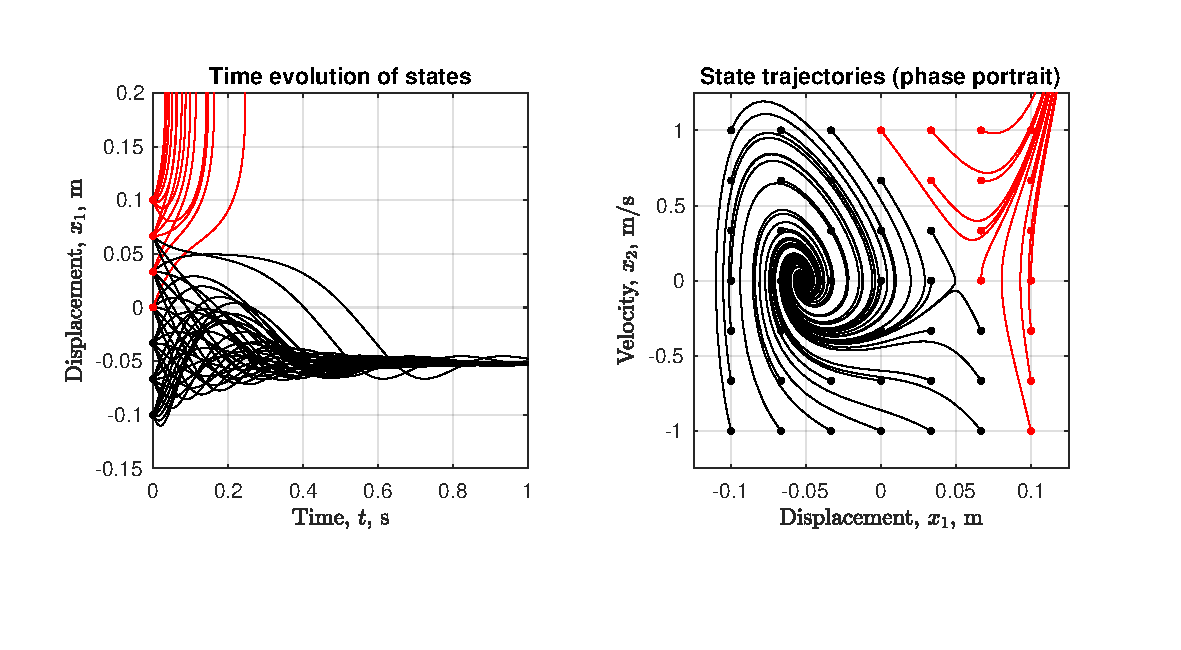
\includegraphics[width=1.2\linewidth]{magspringportrait.pdf}}
\end{frame}

\begin{frame}
\frametitle{Introduction}
In this workshop, we will use a nonlinear system to illustrate the processing of linearisation and then examine the response of the linearised system.
\begin{itemize}
\item Model a nonlinear magnetic spring
\item Visualise its characteristics (same process as last week)
\item Linearise the system
\item Introduce key Matlab commands \texttt{ss}, \texttt{damp}, \texttt{initial}, \texttt{step} \& \texttt{stepplot}, \texttt{bode} \& \texttt{bodeplot}
\end{itemize}

\end{frame}

\SUBCONCEPT{Nonlinear magnetic spring}

\begin{frame}[fragile]
\frametitle{Nonlinear magnetic spring --- force is roughly quadratic}

\begin{columns}

\column{0.5\textwidth}
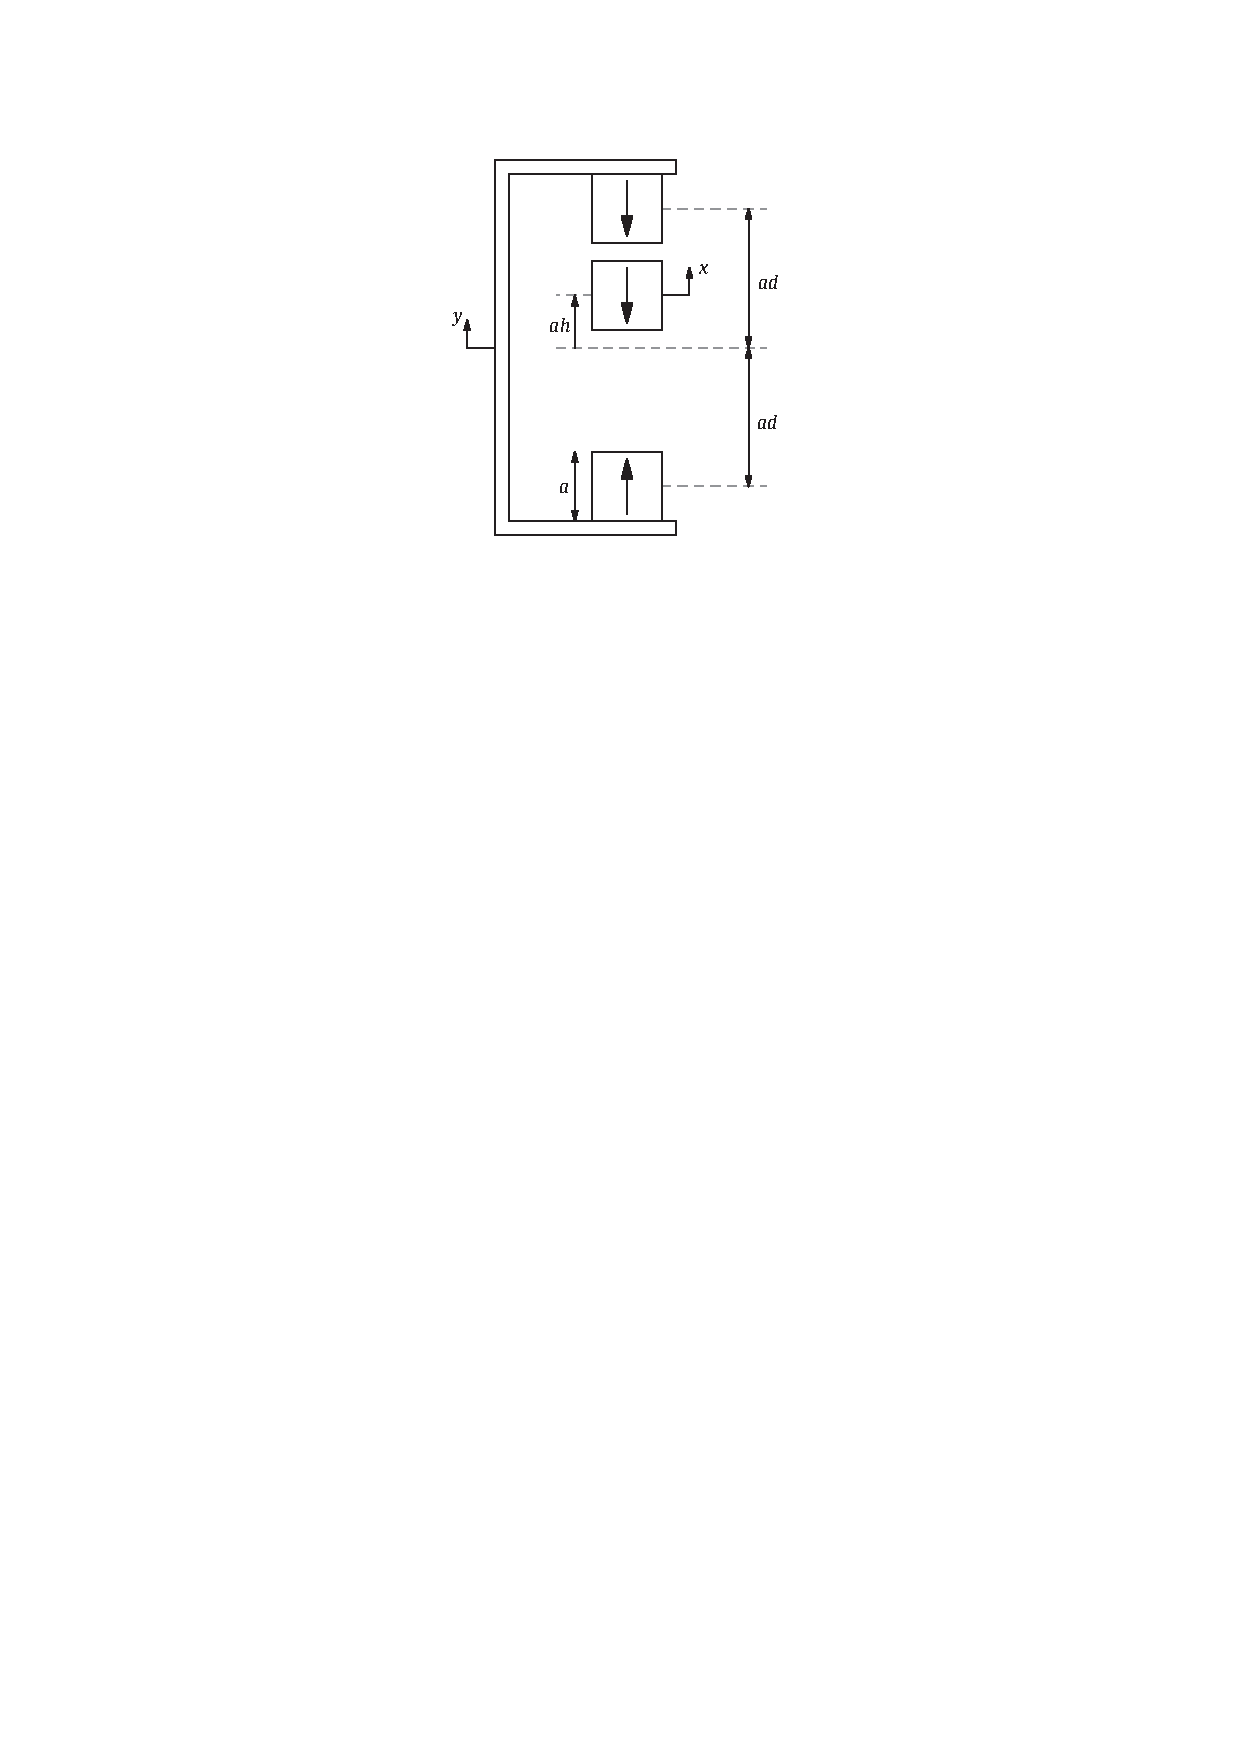
\includegraphics[width=\linewidth]{qzs}

\column{0.5\textwidth}

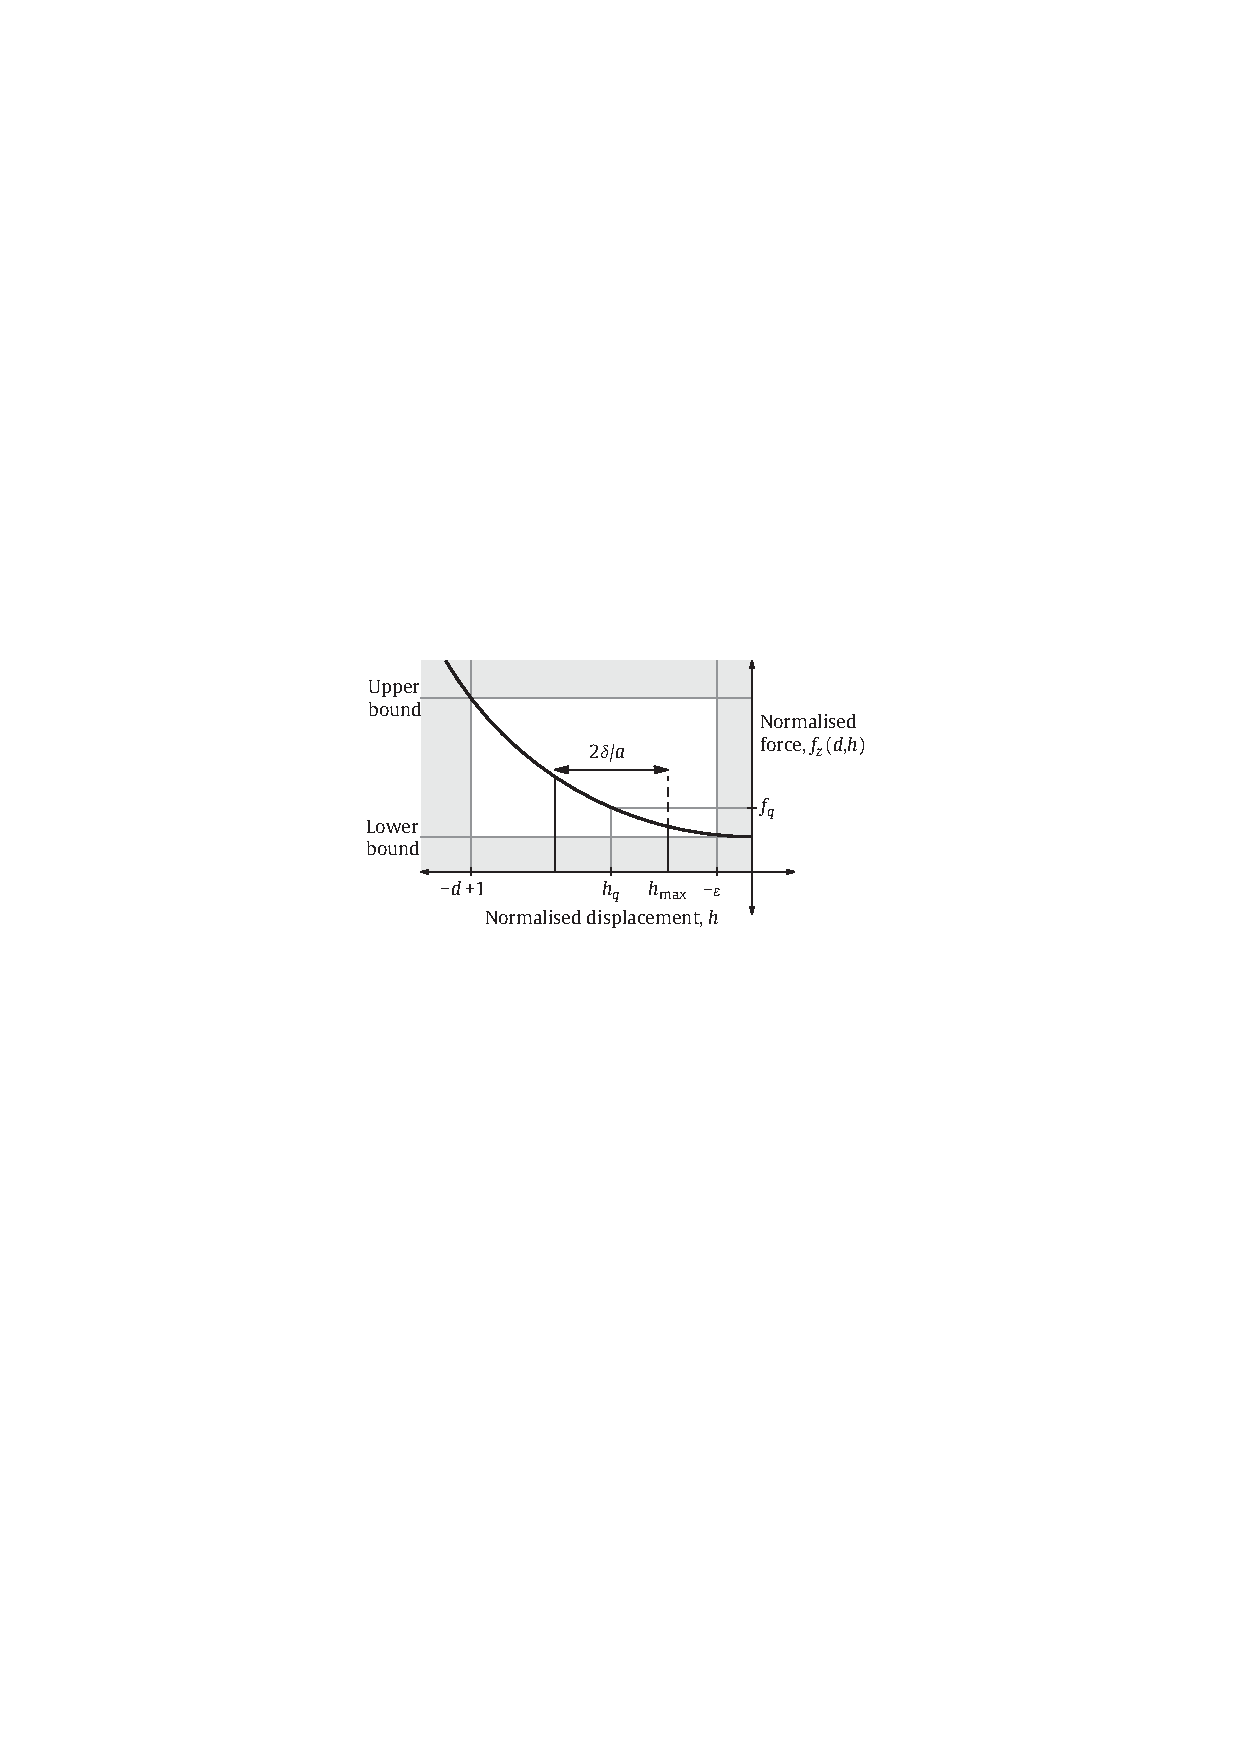
\includegraphics[width=\linewidth]{qzs-forces}%
\begin{itemize}
\item Top magnet pair --- attraction
\item Bottom magnet pair --- repulsion
\item Force curve can be adjusted by shifting the gap between the magnets $g_d = 2ad$
\end{itemize}

\end{columns}

\end{frame}

\begin{frame}
\frametitle{Magnetic forces}

\begin{align}
\sum F_x &= M\ddot x = - c\dot x + f_{spring}(x) - Mg\\
f_{spring}(x)  &= f_{attr}(x) + f_{repl}(x) \\
f_{attr}(x) &= f_{mag}(-g_d/2+x) \\
f_{repl}(x) &= f_{mag}(+g_d/2+x) \\
f_{mag}(x)  &= \frac{3 \mu_0 m_x^2}{2 x^4} \propto \frac{1}{x^4}
\end{align}
\begin{itemize}
\item where all constants and parameters are shown on the following slide
\item note the only parameters to vary are magnet size $a$ and magnet gap $g_d$
\item this is a physically accurate model of two interacting magnetic dipoles; it has good accuracy to model permanent magnets for approx $g_d>4a$
\item (we could add a variable mass but let's keep it simple for now)
\end{itemize}

\end{frame}

\begin{frame}
\frametitle{Simulation parameters}

\begin{tabular}{lcl}
\toprule
Parameter & Symbol & Quantity \\
\midrule
Vacuum permeability & $\mu_0$ & $4\pi\times10^{-7}$ \si{N/A^2} \\
Magnet side length & $a$ & \qty{0.025}{m} \\
Remanence magnetisation & $B_r$ & \qty{1.3}{T} \\
Density & $\rho$ & \qty{7500}{kg/m^3} \\
Viscous damping & $c$ & \qty{1}{kg/m} \\
Gravity & $g$ & \qty{9.81}{m/s^2} \\
\midrule
Magnet gap & $g_d$ & 16a \\
\midrule
Volume & $V$ & $a^3$ \\
Mass & $M$ & $\rho V$ \\
Dipole moment & $m_x$ & $B_r V/\mu_0$\\
\bottomrule
\end{tabular}

\end{frame}

\begin{frame}
\frametitle{Implementation}

\begin{itemize}
\item In this code we will use a structure to hold all of the parameters, as there are quite a few:
\end{itemize}

\includematlab{workshop3.m}{param}

\begin{itemize}
\item These work exactly like you would expect (e.g., you just type \texttt{param.mass} to get the mass) but you can also pass around \texttt{param} itself to other functions.
\end{itemize}

\end{frame}

\begin{frame}

\frametitle{Calculating forces}

\begin{itemize}
\item There's one trick to keep an eye out here; the code needs to be vectorised to allow multiple displacements to be entered as an array of inputs, to calculate an array of  output forces:
\end{itemize}

\includematlab{workshop3.m}{forces}

\begin{itemize}
\item At this point we always plot the graphs to check they look reasonable:
\end{itemize}

\includematlab{workshop3.m}{plot1}

\begin{itemize}
\item Check your understanding: what does an intersection between the horizontal line and the magnetic force curve mean?
\end{itemize}

\end{frame}

\begin{frame}
\frametitle{Understanding the system}

\begin{itemize}
\item The second sanity check is to vary the magnet gap and check how this affects the forces. Does it look reasonable?
\end{itemize}

\includematlab{workshop3.m}{plot2}

\begin{itemize}
\item Check your understanding: what does it mean if there is \emph{no intersection} between the horizontal line and the magnetic force?
\end{itemize}

\end{frame}

\begin{frame}
\frametitle{Implementing the differential equation}

\begin{itemize}
\item As we've seen before, when you have all the system forces all it needs is some wrapper code to tie it together for solving the ODEs numerically.
\item Start with the wrapper:
\end{itemize}

\includematlab{workshop3.m}{msd}

\begin{itemize}
\item Note we have inserted the force equations inside this function to make it all self-contained. This is necessary due to the way Matlab handles function scope.
\item If you need to use many parameters in such functions, you might `break out' the individual parameters into their own variable to shorten the code. E.g. \texttt{M = param.mass;}
\end{itemize}

\end{frame}

\begin{frame}
\frametitle{Solving the ODE}

\begin{itemize}
\item From here it's straightforward to solve the ODE for a single initial condition:
\end{itemize}

\includematlab{workshop3.m}{ode}

\begin{itemize}
\item And you've seen plotting before; be careful with this style of dual axes that the colours are chosen to be colour-blind accessible:
\end{itemize}

\includematlab{workshop3.m}{plot3}

\end{frame}

\SUBCONCEPT{Visualising nonlinear magnetic spring characteristics}

\begin{frame}
\frametitle{Quiver plot --- same as last week}

\includematlab{workshop3.m}{quiv1}

\includematlab{workshop3.m}{quiv2}

\end{frame}

\begin{frame}
\frametitle{Phase plot --- same last last week}

\begin{itemize}
\item Setup:
\end{itemize}
\includematlab{workshop3.m}{phase1}

\begin{itemize}
\item Generate and plot the trajectories:
\end{itemize}
\includematlab{workshop3.m}{phase2}

\end{frame}

\begin{frame}
\frametitle{Phase plot --- same as last week}

\begin{itemize}
\item Don't forget to make the plots pretty:
\end{itemize}

\includematlab{workshop3.m}{phase3}

\begin{itemize}
\item Check your understanding: what is the difference between the red and black curves? How are we automatically detecting the differences between them? What does it tell us about the stability of the system? Can we see this behaviour from the quiver plot, too?
\end{itemize}

\end{frame}

\SUBCONCEPT{Linearisation}


\begin{frame}
\frametitle{Taylor series expansion}
The Taylor series of differentiable function $f$ about point $a$ is:
\begin{align}
f(x) = f(a) + f'(a)(x - a) + \frac{f''(a)}{2!}(x - a)^2 + \cdots
\end{align}
For linearisation, we truncate:
\begin{align}
f(x) \approx f(a) + \alert{f'(a)}(x - a)
\end{align}
Our nonlinear function is:
\begin{align}
f_{mag}(x)  &= \frac{3 \mu_0 m_x^2}{2 x^4} \,, & f_{spring}(x)  &= f_{mag}\bigl(-\tfrac{g_d}{2}+x\bigr) + f_{mag}\bigl(\tfrac{g_d}{2}+x\bigr)
\end{align}
The derivative is:
\begin{align}
f'_{mag}(x)  &= \frac{-6 \mu_0 m_x^2}{x^5} \,, & f'_{spring}(x) &= f'_{mag}\bigl(-\tfrac{g_d}{2}+x\bigr) + f'_{mag}\bigl(\tfrac{g_d}{2}+x\bigr)
\end{align}
\end{frame}

\begin{frame}
\frametitle{Differentiation check}
\begin{itemize}
\item If you are anything like me you will want to check your maths by plotting the derived nonlinear stiffness against the numerical equivalent:
\end{itemize}

\includematlab{workshop3.m}{deriv}

\begin{itemize}
\item This also shows that it is possible to do this step entirely numerically (but be careful about accuracy).
\end{itemize}

\end{frame}

\begin{frame}
\frametitle{Find equilibria}
\begin{itemize}
\item To find the equilibrium points use a numerical root-finder. In other words, use an initial guess to find closest $x_{eq}$ such that:
\end{itemize}
\begin{align}
f_{spring}(x_{eq}) - Mg = 0
\end{align}
\includematlab{workshop3.m}{root}
\begin{itemize}
\item (Based on the quiver plot / phase portrait, we have a good idea that there are two of these and how to get close to them.)
\end{itemize}

\end{frame}

\begin{frame}
\frametitle{Construct linear state space matrices}
Based on the steps above, we can now jump ahead and write down the linear state space equations: (assuming $f$ is an applied input force on the floating mass)
\begin{align}
\dot z &= Az + Bu &
\Matr{ \dot x \\ \ddot x } &= \Matr{ 0 & 1 \\ k_{lin}/M & -c/M } \Matr{ x\\ \dot x } + \Matr{0 \\ 1/M}f
\end{align}
where
\begin{align}
k_{lin} &= f'_{spring}(x_{eq}) = f'_{mag}\bigl(-\tfrac{g_d}{2}+x_{eq}\bigr) + f'_{mag}\bigl(\tfrac{g_d}{2}+x_{eq}\bigr)
\end{align}
We have not explicitly indicated in the notation the change of coordinates so that $x$ is now centred at an equilibrium point and the static forces cancel.

\begin{itemize}
\item \scriptsize Although this slide is a bit hand-wavy, you should think through this process in detail in your own time to make sure you are happy with it.
(The Jacobian Linearisation approach is equivalent to what we've done above.)
\end{itemize}
\end{frame}

\begin{frame}
\frametitle{Matlab implementation}
\alert{We are finally ready to show you Matlab state space matrices.}

\includematlab{workshop3.m}{ss}

\begin{itemize}
\item This defines a linear model for our magnetic spring around the first (stable) equilibrium point
\item Use \texttt{damp(magss1)} to extract the eigenvalues/poles, their frequencies, and damping ratios
\item Use commands like \texttt{step(magss1)} to visualise step responses, etc.
\end{itemize}

\end{frame}

\begin{frame}
\frametitle{Comparing linear and nonlinear responses}
LTI systems in Matlab (whether defined in state space or transfer function form) have a rich set of tools for visualising and analysing their behaviour. Here, let's compare the linear and nonlinear responses to an initial condition:

\includematlab{workshop3.m}{lin}

Change the initial condition (e.g. $5\times$ larger and $5\times$ smaller) --- what do you see?

\end{frame}


\SUBCONCEPT{System response graphs}


\begin{frame}
\frametitle{Step response}

So for this linear system that we have defined, we can now examine the behaviour with a variety of Matlab tools. For example, when the input force provides a step change:

\includematlab{workshop3.m}{step}

\begin{itemize}
\item The \texttt{stepinfo} command provides quantitative metrics which can be used for optimisation, comparison, etc.
\item The \texttt{stepplot} command is intended for visualisation, with options provided for highlighting parts of the graph (you can also right click and explore interactively).
\item There is also \texttt{step} which is better for extracting the raw data from the curves if you wish to draw your own (see example using \texttt{initial} on previous slide).
\end{itemize}

\end{frame}


\begin{frame}
\frametitle{Frequency response}

And this is the steady state response to sinusoidal input vs frequency:

\includematlab{workshop3.m}{frf}

\begin{itemize}
\item The frequency response is one of the most important (perhaps the most important) details of this course --- we will come back to it a lot.
\item This graph shows the response magnitude vs frequency on the top, and the phase vs frequency on the bottom. For now, the magnitude graph is more interesting, focus on that to begin with.
\end{itemize}

\end{frame}

\begin{frame}
\frametitle{Finally\dots}

\begin{itemize}
\item This was a very long road to introduce a few simple Matlab commands right at the end.
\item Nonlinear modelling is critical in mechanical engineering as many systems behave in complex ways --- need to have the tools to simulate and analyse them with good fidelity.
\item As we move on with the course, more and more of our examples will be linear systems only, but remember they are only models.
\item \alert{If you have the energy, now try varying the \texttt{param.gap} term was back in the beginning, and as long as the system remains stable the entire analysis should still `just work' --- this illustrates the power of this style of modelling approach.}
\end{itemize}

\end{frame}

\end{document}




